\chapter{Resultados Preliminares}
\label{cap:04}

Foi desenvolvido um jogo do gênero \textit{farming} com elementos \textit{cozy}, como movimentação livre, progressão por coleta e também cultivo, junto de interações ambientais. Apesar de haver espaço para melhorias e novas funcionalidades, o jogo está operacional, com os principais sistemas implementados.

As seções a seguir detalham os resultados que foram obtidos, focando na parte de desenvolvimento e na interface do jogador.

\section{Desenvolvimento}

\FloatBarrier 
\begin{figure}[!htbp]
	\centering
	\caption{Pastas principais}
	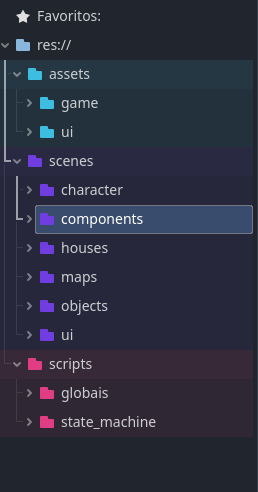
\includegraphics[width=0.3\linewidth]{imagens/Pastas.png}
	\\\textbf{Fonte:} Elaborada pelo autor
	\label{fig:pastas}
\end{figure}
\FloatBarrier


\section{Cronograma do Trabalho}

Segue abaixo o cronograma de trabalho das atividades realizadas e das que serão executadas até a Avaliação Final de TCC.

\textbf{Obs:} Para facilitar, crie o cronograma usando o modelo do Word contido no projeto (imagens/templateCronograma.docx), ou qualquer outro \textit{software}, salve a imagem e atualize o arquivo imagens/cronograma.png.

\FloatBarrier
\begin{figure*}[!htbp]
	\centering
	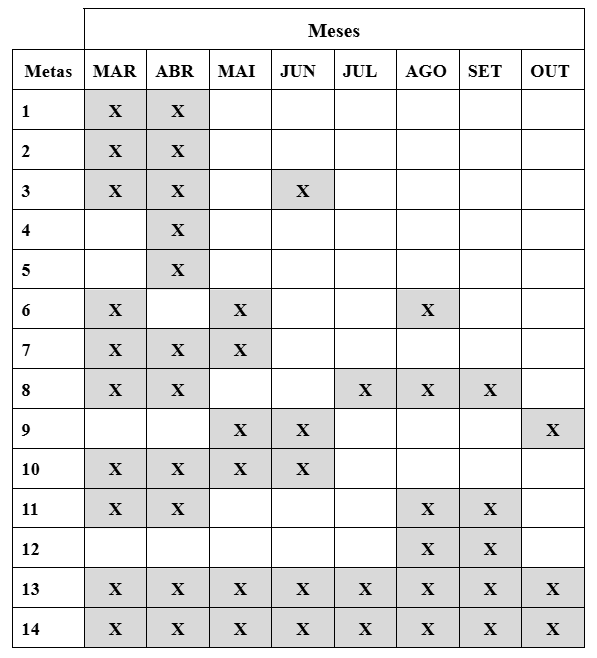
\includegraphics[scale=1]{imagens/cronograma}
\end{figure*}
\FloatBarrier

\begin{enumerate}
	\item Descrição da atividade 1;
	\item Descrição da atividade 2;
	\item Descrição da atividade 3;
	\item Descrição da atividade 4;
	\item Descrição da atividade 5.
\end{enumerate}
